\section{Composite Transfer Function}\label{Sec:Ctf}
We extended our basic raycaster so that it performs compositing of colors and opacities of all voxels along the view ray.
The skeleton code already provided a transfer function editor, so we only needed to concentrate on the compositing aspect.
The idea of compositing is to make layers that are semi transparant visible. 
We can do this by using the following function for each color: 
$$\sum_{i=0}^{n-1} c_{i}\Pi_{j=i+1}^{n-1}(1-\tau_{j})  $$.
When start with n-1 and go back to 1, we can compute the whole sum in linear time. 
Because when we start with n-1, we can save each step of the product.
This means that for every i, we only have to do one multiply to compute the next state of the product.\\
We were interested in what would happen if we compute it the other way around, so we dit not only implement this function: \\
$$\sum_{i=0}^{n-1} c_{i}\Pi_{j=i+1}^{n-1}(1-\tau_{j})  $$. 
We also implemented this function: \\
$$\sum_{i=n-1}^{0} c_{i}\Pi_{j=i-1}^{0}(1-\tau_{j})  $$
\begin{figure}[H]
	\centering
	\begin{subfigure}[t]{0.45\textwidth}
		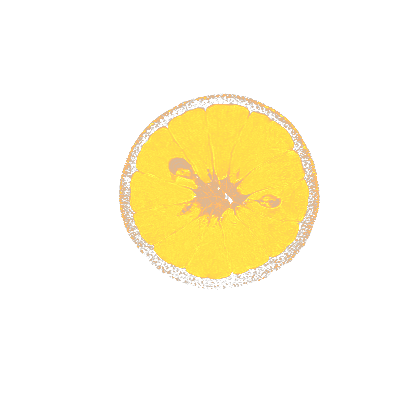
\includegraphics[width=\textwidth]{orange_btf}
		\caption{The orange with the back to front composite function}
	\end{subfigure}
	~%
	\begin{subfigure}[t]{0.45\textwidth}
		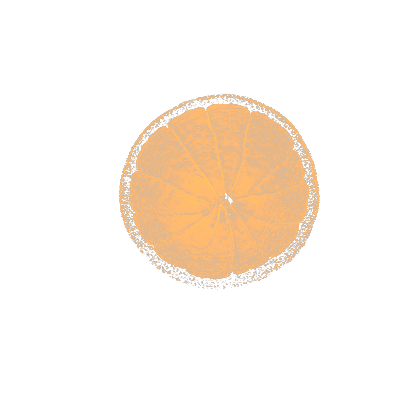
\includegraphics[width=\textwidth]{orange_ftb}
		\caption{The orange with the front to back composite function}
	\end{subfigure}
	
	\caption{A comparison of rendering \texttt{orange.fld} with the front to back and back to front composite transfer functions}
	\label{fig:ctf:comp}
\end{figure}
As you can see in figure~\ref{fig:ctf:comp}, there are major differences between the front to back and back to front composite transfer functions.
In Section~\ref{Sec:Com} we will compare both functions and analyse their differences.




